\input{../preamble.tex}

\SetDate[13/05/2026]

\begin{document}
\pagestyle{fancy}
\fancyhead[L]{Seconde}
\fancyhead[C]{\textbf{Signes et variations}}
\fancyhead[R]{\today}

\subsection*{Automatismes}


\exemulticols{}{
	Considérons les graphes de $f$ et $g$ sur le domaine $\D = [-2,5 ; 2,3]$ ci-contre.

	Remplir les pointillés avec le signe $<$ (inférieur strict), $>$ (supérieur strict), ou $=$ (égal).
	\setlength{\columnseprule}{1pt} 
	\begin{multicols}{2}
\setlength{\abovedisplayskip}{-15pt}
\setlength{\belowdisplayskip}{-15pt}
	\begin{align*}
		f(0,5) &\quad\dots\quad 0 \\
		g(0,5) &\quad\dots\quad 0 \\
		f(0,5)\cdot g(0,5) &\quad\dots\quad 0 \\
		f(-2) &\quad\dots\quad 0 \\
		g(-2) &\quad\dots\quad 0 \\
		f(-2)\cdot g(-2) &\quad\dots\quad 0 
	\end{align*}
	
	\columnbreak
	
	\begin{align*}
		f(1,5)\cdot g(1,5) &\quad\dots\quad 0 \\
		f(0)\cdot g(0) &\quad\dots\quad 0 \\
		f(1)\cdot g(1) &\quad\dots\quad 0 \\
		f(-1,5)\cdot g(-1,5) &\quad\dots\quad 0 \\
		f(2)\cdot g(2) &\quad\dots\quad 0 \\
		f(-1)\cdot g(-1) &\quad\dots\quad 0
	\end{align*}
	\end{multicols}
	%Donner l'ensemble des \mbox{$x \in [-2,5 ; 2,3]$} vérifiant $f(x) = g(x)$.
}{
	\begin{center}
	\begin{tikzpicture}[>=stealth]
		\begin{axis}[xmin = -2.5, xmax=2.3, ymin=-4.1, ymax=4.6, axis x line=middle, axis y line=middle, axis line style=->, grid=both,
			grid style = {opacity=.5},
			x=1.5cm,
			xtick={-3, -2, ..., 2},
			y=20pt,
			clip=true,
			]
			\addplot[no marks, BLUE_E, -, very thick] expression[domain=-2.5:2.3, samples=101]{(x-1)*(x-2)*(x+2)/2}
			node[pos=.5, above]{$\mathcal{C}_f$};
			\addplot[no marks, RED_E, -,  very thick] expression[domain=-2.5:2.3, samples=101]{1/(x-2.5) + 1/(x+2.7) + 2*x}
			node[pos=.75, above]{$\mathcal{C}_g$};
		\end{axis}
	\end{tikzpicture}
	\end{center}
}{exe:f-equals-g}{

	\setlength{\columnseprule}{1pt} 
	\begin{multicols}{2}
\setlength{\abovedisplayskip}{-15pt}
\setlength{\belowdisplayskip}{-15pt}
	\begin{align*}
		f(0,5) &> 0 \\
		g(0,5) &> 0 \\
		f(0,5)\cdot g(0,5) &> 0 \\
		f(-2) &= 0 \\
		g(-2) &< 0 \\
		f(-2)\cdot g(-2) &= 0 
	\end{align*}
	
	\columnbreak
	
	\begin{align*}
		f(1,5)\cdot g(1,5) &< 0 \\
		f(0)\cdot g(0) &= 0 \\
		f(1)\cdot g(1) &< 0 \\
		f(-1,5)\cdot g(-1,5) &< 0 \\
		f(2)\cdot g(2) &= 0 \\
		f(-1)\cdot g(-1) &< 0
	\end{align*}
	\end{multicols}
}


\exemulticols{}{
	Exprimer par lecture graphique les ensembles suivants sous forme d'union d'intervalles.
		\begin{enumerate}[itemsep=25pt]
		% for Natalija :)
			\item $\bigset{ x \in [-3 ; 3] \text{ tq. } f(x) \geq 0}$
			\item $\bigset{ x \in [-3 ; 3] \text{ tq. } g(x) \leq 0}$
			\item $\bigset{ x \in [-3 ; 3] \text{ tq. } f(x) \cdot g(x) \geq 0}$
		\end{enumerate}
	\vfill\null
}{
	\begin{center}
	\begin{tikzpicture}[>=stealth, scale=1]
	\begin{axis}[xmin = -3, xmax=3, ymin=-4, ymax=4, axis x line=middle, axis y line=middle, axis line style=<->, xlabel={}, ylabel={}, xtick = {-4, -3, ..., 4}, ytick = {-4, -3, ..., 4}, grid=both, clip=true]
		
		% (g)
		\addplot[RED_E, very thick, domain =-3:3, samples=50] {(x+1)*x*(x-2)+.5}  node[pos = .77, right=2pt] {$\C_g$};
		
		% (f)
		\addplot[BLUE_E, very thick, domain =-3:3, samples=50] {2.9-1.2*x^2}  node[pos = .41, above=4pt] {$\C_f$};
	\end{axis}
	\end{tikzpicture}
	\end{center}
}{exe:aut0}{
	L'ordonnée du point d'abscisse $x$ appartenant à $\C_f$ est $f(x)$.
	On lit donc son signe en regardant s'il est au-dessus ou en-dessous de l'axe des abscisses.
	
	\begin{enumerate}
		\item On a environ 
			\[ \{ x \in [-3 ; 3] \text{ tq. } f(x) \geq 0\} \approx [-1,5 ; 1,5]. \]
		\item On a environ 
			\[ \{ x \in [-3 ; 3] \text{ tq. } g(x) \leq 0\} \approx [-3 ; -1,2] \cup [1,9 ; 3]. \]
		On est en droit de se demander : comment sait-on que $g(-2) \leq 0$ si on ne peut pas lire sa valeur graphiquement ?
		On suppose en fait ici que $\C_g$ est une courbe continue (tracée sans lever le crayon). 
		Ainsi, si $g(-2)$ était positif, la courbe devrait nécessairement couper l'axe des abscisses, ce qui n'est visiblement pas le cas.
		\item Il y a deux situations dans lesquelles le produit $f(x) \cdot g(x)$ peut être positif : soit $f(x)$ et $g(x)$ sont positifs, soit ils sont tous deux négatifs.
		Graphiquement, on lit que
			\[ \{ x \in [-3 ; 3] \text{ tq. } f(x) \geq 0 \text{ et } g(x) \geq 0 \} \approx [-1,2 ; 0,2], \]
		et que (en faisant à nouveau une hypothèse de continuité)
			\[ \{ x \in [-3 ; 3] \text{ tq. } f(x) \leq 0 \text{ et } g(x) \leq 0 \} \approx [-3 ; -1,6] \cup [1,6 ; 1,9]. \]
		On prend l'union des deux pour obtenir
			\[ \{ x \in [-3 ; 3] \text{ tq. } f(x) \cdot g(x)  \geq 0 \} \approx [-1,2 ; 0,2] \cup [-3 ; -1,6] \cup [1,6 ; 1,9]. \]
	\end{enumerate}
}


\exe{}{
	Pour chacune des fonctions affines $f$ suivantes, donner l'intervalle 
		$ \bigset{ x \in \R \text{ tq. } f(x) \geq 0 }. $
	
	\begin{multicols}{3}
	\begin{enumerate}
		\item $f(x) = x+3$
		\item $f(x) = 3x-10$
		\item $f(x) = x$
		\item $f(x) = -4x-12$
		\item $f(x) = -10x$
		\item $f(x) = 1$
	\end{enumerate}
	\end{multicols}
}{exe:1}{
	\begin{enumerate}
		\item 
		L'inégalité $x+3 \geq 0$ est équivalente à $x \geq -3$.
		On obtient donc 
			\[ \{ x \in \R \text{ tq. } x+ 3 \geq 0 \} = \{ x \in \R \text{ tq. }x \geq -3 \} = [-3 ; \pinfty[. \]
		\item 
			\[ \left[ \dfrac{10}3 ; \pinfty \right[ \]
		\item
			\[ [0 ; \pinfty[ \]
		\item
		L'inégalité $-4x - 12 \geq 0$ est équivalente à $-4x \geq 12$.
		Pour continuer, on multiplie par $-\dfrac14$ qui est négatif, ce qui change donc le sens de l'inégalité : $x \leq -3$.
		On obtient donc
			\[ ]\minfty ; -3]. \]
		\item
			\[ ]\minfty ; 0] \]
		\item 
			Tous les $x\in\R$ vérifie que $f(x) \geq 0$ car $1 \geq 0$ est toujours vrai.
			Donc 
			\[ \{ x \in \R \text{ tq. } 1 \geq 0 \} = \R. \]
	\end{enumerate}

}


\subsection*{Exercices}




\exe{}{
	À l'aide de l'exercice \ref{exe:1}, donner le domaine de définition de chaque fonction suivante.
	
	\begin{multicols}{3}
	\begin{enumerate}
		\item $f(x) = \sqrt{x+3}$
		\item $g(x) = \sqrt{3x-10}$
		\item $h(x) = \sqrt{-4x-12}$
	\end{enumerate}
	\end{multicols}

}{exe:2}{
	Le domaine de définition est le plus grand domaine sur lequel une fonction est bien définie.
	Ici, la seule chose qui peut se mal passer est qu'on demande à $f$ de calculer une racine carrée d'un nombre négatif.
	Ceci n'est pas possible car $x^2 \geq 0$ pour tout $x\in\R$, donc si on souhaite calculer $\sqrt{a}$ vérifiant $\sqrt{a}^2 = a$ par définition, on a nécessairement $a\geq0$.
	Par exemple, $\sqrt{-1}$ ne peut pas être un nombre réel, sinon $\sqrt{-1}^2 = -1$, et un carré serait négatif !
	
	On impose donc que l'expression sous une racine carrée soit positive ou nulle, et on prend tous les réels vérifiant cette propriété.
	\begin{enumerate}
		\item
			\[ \D_f = \{ x \in \R \text{ tq. } x + 3 \geq 0 \} = [-3; \pinfty[, \]
		d'après l'exercice \ref{ex:1}.
		\item
			\[ \D_f = \{ x \in \R \text{ tq. } 3x- 10 \geq 0 \} = \left[ \dfrac{10}3 ; \pinfty \right[, \]
		d'après l'exercice \ref{ex:1}.
		\item
			\[ \D_f = \{ x \in \R \text{ tq. } -4x-12 \geq 0 \} = ]\minfty; -3], \]
		d'après l'exercice \ref{ex:1}.
	\end{enumerate}
}



\exe{}{
	À l'aide de l'exercice \ref{exe:1} remplir les tableaux de signes ci-dessous et donner
		\begin{align*}
			\{ x \in \R \text{ tq. } f(x) \geq 0 \}, && \{ x \in \R \text{ tq. } g(x) \leq 0 \}, && \{ x \in \R \text{ tq. } h(x) \geq 0 \}
		\end{align*}
	sous forme d'union d'intervalles.
	
	\begin{center}
	\begin{tikzpicture}
		\tkzTabInit
		 %[lgt=3,espcl=1.5]
		 [lgt=5]
	       		{$x$ / 1 , $x+3$ / 1, $3x-10$ / 1 , $f(x) = (x+3)(3x-10)$ / 1}
	       		{$\minfty$,,,$\pinfty$}
		
	\end{tikzpicture}
	
	\begin{tikzpicture}
		\tkzTabInit
		 %[lgt=3,espcl=1.5]
		 [lgt=5]
	       		{$x$ / 1 , $x$ / 1, $-4x-12$ / 1 , $g(x) = x(-4x-12)$ / 1}
	       		{,,,}
	       		
	\end{tikzpicture}
	
	
	\begin{tikzpicture}
		\tkzTabInit
		 %[lgt=3,espcl=1.5]
		 [lgt=5]
	       		{$x$ / 1 , $x+3$ / 1, $-10x$ / 1 , $3x-10$ / 1 , $h(x) = -10x(x+3)(3x-10)$ / 1}
	       		{,, , ,}
	   
	\end{tikzpicture}
	\end{center}
}{exe:3}{
	\begin{center}
	\begin{tikzpicture}
		\tkzTabInit
		 %[lgt=3,espcl=1.5]
		 [lgt=5]
	       		{$x$ / 1 , $x+3$ / 1, $3x-10$ / 1 , $f(x) = (x+3)(3x-10)$ / 1}
	       		{$\minfty$,$-3$, $\dfrac{10}3$,$\pinfty$}
		
		\tkzTabLine
			{,-,z,+,,+}
		\tkzTabLine
			{,-,,-,z,+}
		\tkzTabLine
			{,+, z, -, z, +}
	\end{tikzpicture}
	
	\begin{tikzpicture}
		\tkzTabInit
		 %[lgt=3,espcl=1.5]
		 [lgt=5]
	       		{$x$ / 1 , $x$ / 1, $-4x-12$ / 1 , $g(x) = x(-4x-12)$ / 1}
	       		{ $\minfty$ , $-3$ , $0$ , $\pinfty$ }
	       		
		\tkzTabLine
			{,-,z,+,,+}
		\tkzTabLine
			{,+,,+,z,-}
		\tkzTabLine
			{,-, z, +, z, -}
	\end{tikzpicture}
	
	
	\begin{tikzpicture}
		\tkzTabInit
		 %[lgt=3,espcl=1.5]
		 [lgt=5]
	       		{$x$ / 1 , $x+3$ / 1, $-10x$ / 1 , $3x-10$ / 1 , $h(x) = -10x(x+3)(3x-10)$ /1}
	       		{ $\minfty$ , $-3$ ,  $0$ ,  $\dfrac{10}3$ , $\pinfty$ }
	       		
		\tkzTabLine
			{,-,z,+,,+,,+}
		\tkzTabLine
			{,+,,+,z,-,,-}
		\tkzTabLine
			{,-,,-,, -,z,+}
		\tkzTabLine
			{,+,z,-,z, +,z,-}
	\end{tikzpicture}
	\end{center}


	On remplit le tableau de signe en calculant d'abord quand chaque fonction affine s'annule : c'est exactement quand elle change de signe (du positif vers le négatif, ou l'inverse).
	
	Par exemple, $x+3$ s'annule en $x=-3$, et l'exercice \ref{ex:1} donne que $x+3$ est positif après $-3$, est donc nécessairement négatif avant.
	On fait idem pour $3x-10$, qui s'annule en $\dfrac{10}3$, et qui est positif après, et négatif avant.
	
	Le signe du produit $f(x) = (x+3)(3x-10)$ est déduit du signe des facteurs, à l'aide des règles ``positif $\times$ positif = positif ; négatif $\times$ négatif = positif ; positif $\times$ négatif = négatif''.
	De plus, lorsqu'un des deux facteurs des nul, le produit est forcément nul, multiplier par zéro donne toujours zéro.
	
	Le deuxième tableau est similaire, en faisant attention au fait que le signe de $-4x-12$ est positif puis négatif (cf. exercice \ref{ex:1}).
	Ceci est en fait dû au fait qu'on ait multiplié par $-\dfrac14$ lors de la résolution de $-4x-12 \geq 0$.
	Le signe du coefficient directeur $a$ de la fonction affine donne donc l'allure de la droite associée : si $a>0$, la droite monte du négatif vers le positif en passant par $0$, et si $a <0$, la droite descend du positif vers le négatif en passant par $0$.
	
	Le cas $a=0$ est le cas de la fonction constante, dont l'étude de signe n'est pas très intéressante.
}



\exe{}{
	À l'aide de l'exercice \ref{exe:3}, donner le domaine de définition de la fonction
		\[ f(x) = \sqrt{-10x(x+3)(3x-10)}. \]
}{exe:4}{
	La seul contrainte à poser sur $x$ est que l'expression sous la racine soit positive ou nulle.
		\[ \D_f = \{ x \in \R \text{ tq. } -10x(x+3)(3x-10) \geq 0 \}. \]
	Or la dernière ligne du dernier tableau de signes de l'exercice \ref{ex:4} nous donne exactement les intervalles où $h(x) = -10x(x+3)(3x-10)$ est positive ou nulle :
		\[ \D_f = ]\minfty ; -3] \cup \left[0 ; \dfrac{10}3 \right]. \]
}


\exe{}{
	On souhaite connaître pour quels $x\in\D_f$ l'inégalité suivante est vérifée.
		\[ f(x) = \dfrac{2x+1}{7x^2 - 20x - 3} \geq 0 \]
	
	\begin{enumerate}
		\item Montrer que $7x^2 - 20x - 3 = (x-3)(7x+1)$.
		\item En déduire les valeurs interdites à $f$ et donc le domaine de définition $\D_f$.
		\item Remplir le tableau de signes ci-dessous.
		\item Exprimer $\{ x \in \D_f \text{ tq. } f(x) \geq 0 \}$ sous forme d'union d'intervalles.
	\end{enumerate}
	
	
	\begin{center}
	\begin{tikzpicture}
		\tkzTabInit
		 %[lgt=3,espcl=1.5]
	       		{$x$ / 1, $x-3$ / 1 , $7x+1$ / 1, $2x+1$ / 1 , $f(x)$ / 1}
	       		{,, , ,}
	       		
	\end{tikzpicture}
	\end{center}
}{exe:5}{
	\begin{enumerate}
		\item 
		Par double distributivité,
			\[ (x-3)(7x+1) = x^2 \cdot (7) + x \cdot (1 - 21) + (-3) = 7x^2 - 20x - 3. \]
		\item
		Il n'y a pas de racine carrée dans l'expression de $f$ : la seule opération illégale est la division par zéro.
		Le dénominateur $(x-3)(7x+1)$ est nul lorsqu'un des deux facteur est nul, c'est-à-dire lorsque $x=3$ ou $x= -\dfrac17$.
		Par conséquent, $\D_f = \R - \left\{ 3 ; -\dfrac17 \right\}$.
		
		\item 
		Dans la dernière ligne, on note par les doubles barres les valeurs interdites à $f$.
		Lorsque le numérateur $2x+1$ est nul, $f$ est bien nulle, mais $f$ n'est pas définie aux $x$ pour lesquels le dénominateur s'annule.
		\item 
			\[ \{ x \in \D_f \text{ tq. } f(x) \geq 0 \} = \left[ -\dfrac12 ; -\dfrac17 \right[ \cup ]3 ; \pinfty[. \]
		Les valeurs interdites $-\frac17$ et $3$ ne sont pas incluses car elles n'appartiennent pas à $\D_f$, ensemble dans lequel on pioche nos $x$.
	\end{enumerate}
	
	\begin{center}
	\begin{tikzpicture}
		\tkzTabInit
		 %[lgt=3,espcl=1.5]
	       		{$x$ / 1, $x-3$ / 1 , $7x+1$ / 1, $2x+1$ / 1 , $f(x)$ / 1}
	       		{ $\minfty$ , $-\dfrac12$ ,  $-\dfrac17$ ,  $3$ , $\pinfty$ }
	       		
		
		\tkzTabLine
			{,-,,-,,-,z,+}
		\tkzTabLine
			{,-,,-,z,+,,+}
		\tkzTabLine
			{,-,z,+,,+,,+}
		\tkzTabLine
			{,-,z,+,d, -,d,+}
		
	\end{tikzpicture}
	\end{center}
}



\exe{}{
	Pour chaque propriété, donner une fonction $f$ sur $\R$ non identiquement nulle la vérifiant.
	\begin{multicols}{2}
	\begin{enumerate}
		\item $f$ s'annule en $1$.
		\item $f$ s'annule en $-10$.
		\item $f$ s'annule en $0$.
		\item $f$ s'annule en $-10$ et en $1$.
		\item Les zéros de $f$ sont $2, -3, \frac27$, et $0$.
	\end{enumerate}
	\end{multicols}
}{exe:6}{
	La fonction identiquement nulle $f(x) = 0$ n'est bien sûr pas autorisée sinon l'exercice n'a pas d'intérêt !
	\begin{enumerate}
		\item $f(x) = x-1$ fonctionne ainsi que $f(x) = 3(x-1)$, ou $f(x) = -(x-1) = 1-x$.
		\item $f(x) = x+10$ fonctionne, ainsi que $f(x) = (x+10)(x-1)$, et tous ses multiples.
		\item $f(x) = x$ ou $f(x) = 500x$.
		\item $f(x) = (x+10)(x-1) = x^2 +9x -10$.
		\item $f(x) = (x-2)(x+3)(x-\frac27)x$.
	\end{enumerate}

}


\exe{}{
	On souhaite connaître les solutions de l'équation du deuxième degré d'inconnue $x\in\R$ :
		\begin{align}
			22x^2 - 125x + 22  = 0. \label{eq:1}
		\end{align}
	\begin{enumerate}
		\item Montrer que $22x^2 - 125x + 22 = (2x-11)(11x-2)$.
		\item En déduire l'ensemble des solutions de l'équation \eqref{eq:1}.
	\end{enumerate}
}{exe:7}{
	\begin{enumerate}
		\item On part toujours de la forme factorisée qu'on développe par double distributivité :
			\[ (2x - 11)(11x - 2) = 22x^2 - 4x - 121x + 22 = 22x^2 - 125x + 22. \]
		\item On utilise que le produit est nul si est seulement si un des deux facteurs est nul.
		L'ensemble des solutions de \eqref{eq:1} est donc $\left\{ \dfrac{11}2 ; \dfrac2{11} \right\}$.
	\end{enumerate}
}


\exe{}{
	On souhaite connaître les solutions de l'équation du troisième degré d'inconnue $x\in\R$ :
		\begin{align}
			4x^3 - 6x^2 - 2x + 3  = 0. \label{eq:2}
		\end{align}
	\begin{enumerate}
		\item Montrer que $4x^3 - 6x^2 - 2x + 3 = (2x-3) \left(2x^2-1\right)$.
		\item En déduire l'ensemble des solutions de l'équation \eqref{eq:2}.
	\end{enumerate}
}{exe:8}{

	\begin{enumerate}
		\item On part toujours de la forme factorisée qu'on développe par double distributivité.
		On utilise aussi que $x^2 \cdot x = x \cdot x \cdot x = x^3$.
			\[ (2x - 3)(2x^2 - 1) = 4x^3 - 2x -6x^2 + 3. \]
		\item On utilise que le produit est nul si est seulement si un des deux facteurs est nul.
		Or l'équation $2x^2 - 1 = 0$ est équivalente à $x^2 = \dfrac12$.
		En prenant la racine et en utilisant que $\sqrt{x^2} = |x|$, on obtient
			\[ |x| = \sqrt{\dfrac12} = \dfrac1{\sqrt2}. \]
		Les deux valeurs $\pm \dfrac1{\sqrt2}$ (notation $\pm$ pour \og plus ou moins \fg) sont donc solutions.
		On en déduit que l'ensemble des solutions de \eqref{eq:2} est $\left\{ \dfrac32 ; \pm \dfrac1{\sqrt2} \right\} = \left\{ \dfrac32 ; \dfrac1{\sqrt2} ; - \dfrac1{\sqrt2} \right\}$
	\end{enumerate}

}


%\exe{}{
%	On souhaite connaître les solutions de l'équation du quatrième degré d'inconnue $x\in\R$ :
%		\begin{align}
%			16x^4 - 24x^2 + 9  = 0. \label{eq:3}
%		\end{align}
%	\begin{enumerate}
%		\item Montrer que $16x^4 - 24x^2 + 9 = \left(4x^2-3\right)^2$.
%		\item En déduire l'ensemble des solutions de l'équation \eqref{eq:3}.
%	\end{enumerate}
%}{exe:9}{
%
%	\begin{enumerate}
%		\item On part toujours de la forme factorisée qu'on développe à l'aide de l'identité remarquable $(a-b)^2 = a^2 + b^2 -2ab$.
%		On utilise aussi que $(x^2)^2 = x^2 \cdot x^2 = x\cdot x\cdot x\cdot x = x^4$.
%			\[ (4x^2 - 3)^2 = (4x^2)^2 + 3^2 - 2\cdot(4x^2)\cdot3 = 16x^4 + 9 -24x^2. \]
%		\item On utilise que le produit est nul si est seulement si un des deux facteurs est nul.
%		Ici, les deux facteurs sont les mêmes, car $(4x^2 - 3)^2 = (4x^2 - 3)(4x^2 - 3)$, donc on se remet à résoudre $(4x^2 - 3) = 0$.
%		Ceci est équivalent à $x^2 = \dfrac34$, et donc l'ensemble des $x$ vérifiant \eqref{eq:3} est donné par $\left\{ \pm \sqrt{\dfrac34} \right\} = \left\{ \pm \dfrac12\sqrt{3} \right\}= \left\{ \dfrac12\sqrt{3} ;  -\dfrac12\sqrt{3} \right\}$.
%	\end{enumerate}
%
%}


\exe{}{
	\begin{enumerate}
		\item Esquisser la courbe représentative de la fonction affine $f(x) =3x - 2$ sur le domaine $\D = [-10 ; 12]$.
		\item Remplir le tableau de variations et de signes ci-dessous.
	\end{enumerate}
	
	\begin{center}
	\begin{tikzpicture}
		\tkzTabInit
		 %[lgt=3,espcl=1.5]
	       		{$x$ / 1 , Variation de $3x-2$ / 2, Signe de $3x-2$ / 1}
	       		{,,,,}
	\end{tikzpicture}
	\end{center}
}{exe:10}{

	\begin{center}
	\begin{tikzpicture}
		\tkzTabInit
		 %[lgt=3,espcl=1.5]
	       		{$x$ / 1 , Variation de $3x-2$ / 2, Signe de $3x-2$ / 1}
	       		{  $-10$ ,,  $\dfrac23$ ,,  $12$ }
	       	
		\tkzTabVar
			{-/$-32$, R/, R/, R/, +/$34$}
		\tkzTabIma
			{1}{5}{3}{0}
		\tkzTabLine
			{,,-,,z,,+}
	\end{tikzpicture}
	\end{center}

}


\exe{}{
	\begin{enumerate}
		\item Esquisser la courbe représentative de la fonction affine $f(x) = -6x - 2$ sur le domaine $\D = [-10 ; 8]$.
		\item Remplir le tableau de variations et de signes ci-dessous.
	\end{enumerate}
	
	\begin{center}
	\begin{tikzpicture}
		\tkzTabInit
		 %[lgt=3,espcl=1.5]
	       		{$x$ / 1 , Variation de $-6x-2$ / 2, Signe de $-6x-2$ / 1}
	       		{,,,,}
	\end{tikzpicture}
	\end{center}
}{exe:11}{

	\begin{center}
	\begin{tikzpicture}
		\tkzTabInit
		 %[lgt=3,espcl=1.5]
	       		{$x$ / 1 , Variation de $-6x-2$ / 2, Signe de $-6x-2$ / 1}
	       		{  $-10$ ,,  $-\dfrac13$ ,,  $8$ }
	       	
		\tkzTabVar
			{+/$58$, R/, R/, R/, -/$-50$}
		\tkzTabIma
			{1}{5}{3}{0}
		\tkzTabLine
			{,,+,,z,,-}
		
	\end{tikzpicture}
	\end{center}
}


\exe{}{
	\begin{enumerate}
		\item Esquisser la courbe représentative de la fonction affine $f(x) = -3$ sur le domaine $\D = [-12 ; -5]$.
		\item Remplir le tableau de variations et de signes ci-dessous.
	\end{enumerate}
	
	\begin{center}
	\begin{tikzpicture}
		\tkzTabInit
		 %[lgt=3,espcl=1.5]
	       		{$x$ / 1 , Variation de $-3$ / 2, Signe de $-3$ / 1}
	       		{,,,,}
	       	
	\end{tikzpicture}
	\end{center}
}{exe:12}{
	\begin{center}
	\begin{tikzpicture}
		\tkzTabInit
		 %[lgt=3,espcl=1.5]
	       		{$x$ / 1 , Variation de $-3$ / 2, Signe de $-3$ / 1}
	       		{  $-12$ ,,,,  $-5$ }
	       	
		\tkzTabVar
			{+/$-3$, R/, R/, R/,+/$-3$}
		\tkzTabLine
			{,,,,-,,}
	\end{tikzpicture}
	\end{center}
}

\exe{}{
	Remplir approximativement les tableaux ci-dessous à l'aide des graphes de $\C_f$ et $\C_g$ sur le domaine $\D = [-11; -2,5]$.
	
	\begin{center}
	\begin{tikzpicture}[scale=1]
		\begin{axis}[xmin = -11, xmax=-2.5, ymin=-4.3, ymax=3.5, axis x line=middle, axis y line=middle, axis line style=->, grid=both, ytick={-4,-3,...,2,3}, xtick={-11, -10,...,-4,-3},
    every y tick label/.style={
        anchor=near yticklabel opposite,
        xshift=0.2em,
    }]
    			%f de l'éval f° affines
			\addplot[no marks, myb, -, very thick] expression[domain=-11:-8, samples=50]{5*(x+10)*(x^3 - 300*x - 1920)/80} 
			node[pos=.6, right]{$\mathcal{C}_f$};
			\addplot[no marks, myb, -, very thick] expression[domain=-8:-6, samples=2]{5*(x/2 + 3.2)};
			\addplot[no marks, myb, -, very thick] expression[domain=-6:-5, samples=50]{5*((x+5.5)^2 - 0.5^2 + 0.2)};
			\addplot[no marks, myb, -, very thick] expression[domain=-5:-2.5, samples=2]{5*0.2};
			
			% g sinus
			\addplot[no marks, myr, -, very thick] expression[domain=-11:-2.5, samples=500]{2*sin(x*60)}
			node[pos=.75, above]{$\mathcal{C}_g$};
		\end{axis}
	\end{tikzpicture}
	
	\begin{tikzpicture}
		\tkzTabInit
		 [lgt=3,espcl=2]
	       		{$x$ / 1 , Signe de $f(x)$ / 1}
	       		{,,,,,,}
	\end{tikzpicture}
	%\vfill
	\begin{tikzpicture}
		\tkzTabInit
		 [lgt=3,espcl=2]
	       		{$x$ / 1 , Variation de $f(x)$ / 2}
	       		{,,,,,,}
	\end{tikzpicture}
	%\vfill
	\begin{tikzpicture}
		\tkzTabInit
		 %[lgt=3,espcl=1.5]
	       		{$x$ / 1 , Signe de $g(x)$ / 1}
	       		{,,,,}
	\end{tikzpicture}
	%\vfill
	\begin{tikzpicture}
		\tkzTabInit
		[lgt=3,espcl=3]
	       		{$x$ / 1 , Variation de $g(x)$ / 2}
	       		{,,,,}
	\end{tikzpicture}
	\end{center}
	
}{exe:13}{
	\begin{center}
	\begin{tikzpicture}[scale=1]
		\begin{axis}[xmin = -11, xmax=-2.5, ymin=-4.3, ymax=3.5, axis x line=middle, axis y line=middle, axis line style=->, grid=both, ytick={-4,-3,...,2,3}, xtick={-11, -10,...,-4,-3},
    every y tick label/.style={
        anchor=near yticklabel opposite,
        xshift=0.2em,
    }]
    			%f de l'éval f° affines
			\addplot[no marks, myb, -, very thick] expression[domain=-11:-8, samples=50]{5*(x+10)*(x^3 - 300*x - 1920)/80} 
			node[pos=.6, right]{$\mathcal{C}_f$};
			\addplot[no marks, myb, -, very thick] expression[domain=-8:-6, samples=2]{5*(x/2 + 3.2)};
			\addplot[no marks, myb, -, very thick] expression[domain=-6:-5, samples=50]{5*((x+5.5)^2 - 0.5^2 + 0.2)};
			\addplot[no marks, myb, -, very thick] expression[domain=-5:-2.5, samples=2]{5*0.2};
			
			% g sinus
			\addplot[no marks, myr, -, very thick] expression[domain=-11:-2.5, samples=500]{2*sin(x*60)}
			node[pos=.75, above]{$\mathcal{C}_g$};
		\end{axis}
	\end{tikzpicture}
	
	\begin{tikzpicture}
		\tkzTabInit
		 [lgt=3,espcl=2]
	       		{$x$ / 1 , Signe de $f(x)$ / 1}
	       		{ $-11$ , $-10$ , {$-8,4$} , {$-6,5$} ,  {$-5,8$} ,  {$-5,3$} ,  {$-2,5$} }
	       	
		\tkzTabLine
			{,-,z,+,z,-,z,+,z,-,z,+}
		
	\end{tikzpicture}
	%\vfill
	\begin{tikzpicture}
		\tkzTabInit
		 [lgt=3,espcl=2]
	       		{$x$ / 1 , Variation de $f(x)$ / 2}
	       		{ $-11$ , ${-9,1}$ , {$-8$} , {$-6$} ,  {$-5,5$} ,  {$-5$} ,  {$-2,5$} }
	       	
		\tkzTabVar
			{-/$-3$, +/${3,1}$, -/$-4$, +/$1$, -/${-0,2}$, +/$1$, +/$1$}
		
	\end{tikzpicture}
	%\vfill
	\begin{tikzpicture}
		\tkzTabInit
		 %[lgt=3,espcl=1.5]
	       		{$x$ / 1 , Signe de $g(x)$ / 1}
	       		{ $-11$ , $-9$ , $-6$ , $-3$ ,  {$-2,5$} }
	       	
		\tkzTabLine
			{,+,z,-,z,+,z,-}
		
	\end{tikzpicture}
	%\vfill
	\begin{tikzpicture}
		\tkzTabInit
		[lgt=3,espcl=3]
	       		{$x$ / 1 , Variation de $g(x)$ / 2}
	       		{ $-11$ , ${-10,5}$ , {$-7,5$} , {$-4,5$} ,  {$-2,5$} }
	       	
		\tkzTabVar
			{-/{$1,8$},+/{$2$}, -/{$-2$}, +/{$2$}, -/{$-1$}}
		
	\end{tikzpicture}
	\end{center}

}



\exe{}{
	Pour chaque proposition suivante, démontrer qu'elle est \underline{toujours vraie} ou montrer qu'elle \underline{peut être fausse} avec un contre-exemple.
	$f, g, h, F$ et $G$ sont des fonctions définies sur $\R$.
	\begin{enumerate}
		\item Si $f$ est affine et admet deux racines distinctes, alors $f(x) = 0$ pour tout $x\in\R$.
		\item Si $g(x) \geq 0$ pour tout $x\in\R$, alors $g$ n'admet aucune racine.
		\item Si $h(x) > 0$ pour tout $x\in\R$, alors $h$ n'admet aucune racine.
		\item Si $F$ n'admet aucune racine, alors $F(x) > 0$ pour tout $x\in\R$.
		\item $G(x) = (x-3)^2 (x-5)^2$ est toujours positive est admet exactement deux racines distinctes.
	\end{enumerate}
}{exe:14}{

	\begin{enumerate}
		\item 
		C'est vrai. 
		Si $f$ est affine et admet deux racines distinctes, alors sa courbe représentative est une droite qui intersecte deux fois l'axe des abscisses en deux endroits différents.
		$\C_f$ et l'axe des abscisses sont donc confondues et on a bien $f(x) = 0$ pour tout $x\in\R$.
		
		Algébriquement, on a $(x_A ; 0), (x_B ; 0) \in \C_f$ pour $x_A \neq x_B$.
		La formule du coefficient directeur donne $a = 0$, et une appartenance donne $b=0$.
		
		\item 
		C'est faux : être positif ou nul n'empêche pas d'être nul.
		On pourra prend la fonction carré $f(x) = x^2$ comme contre-exemple : $f(x) \geq 0$ pour tout $x\in\R$ et pourtant $f$ admet $0$ pour racine car $f(0) = 0$.
		
		\item 
		C'est vrai : être strictement positif empêche d'être nul. 
		C'est bien la différence entre la positivité stricte ($>$) et large ($\geq$).
		
		\item 
		C'est faux : si $F$ ne s'annule jamais, elle n'est pas nécessairement toujours strictement positive car elle pourrait aussi être toujours strictement négative !
		Prenons par exemple $f(x) = -1 -x^2$ qui vérifie $f(x) \leq -1 < 0$ pour tout $x\in\R$ réel.
		
		\item 
		C'est vrai.
		Un carré est toujours positif, donc $G(x)$ est le produit de deux positifs et est positif.
		En outre, si $G(x) = 0$, alors $(x-3)^2 = 0$ ou $(x-5)^2 = 0$.
		Il suit que $x=3$ ou $x=5$, et ce sont les deux seules racines de $G$.
		
	\end{enumerate}

}



\exe{}{
	Pour chaque proposition suivante, dire si elle est \underline{toujours vraie} ou si elle \underline{peut être fausse} à l'aide du tableau de variations suivant.
	
	\begin{center}
\def\arraystretch{1.5}
\setlength\tabcolsep{6pt}
	\begin{tikzpicture}
		\tkzTabInit
		 [lgt=3,espcl=1.5]
	       		{$x$ / 1 , Variation de $f(x)$ / 2}
	       		{7,$a$,11,$b$,$c$,28,$d$,31}
			
		\tkzTabVar
			{-/, +/,-/$-45$,R/,R/,+/$20$, R/, -/$-30$}
		\tkzTabIma
			{1}{2}{1}{$30$}
%		\tkzTabIma
%			{3}{6}{3}{25}
%		\tkzTabIma
%			{3}{6}{6}{70}
			
	\end{tikzpicture}
	\begin{tabular}{|c|c|c|} \hline
		Proposition & Vrai & Faux \\ \hline
		$f(a) = 35$ & &  \\ \hline
		$f(a) > 30$ &  & \\ \hline
		$f(b) \leq 20$ &  & \\ \hline
		$f(a) > f(b)$ &  & \\ \hline
	\end{tabular}	
	\hfill
	\begin{tabular}{|c|c|c|} \hline
		Proposition & Vrai & Faux \\ \hline
		$f(b) < f(c)$ &  & \\ \hline
		$f(c) < f(a)$ &  & \\ \hline
		$f(c) = 19$ & &  \\ \hline
		$f(c) < 30$ &  & \\ \hline
	\end{tabular}
	\hfill
	\begin{tabular}{|c|c|c|} \hline
		Proposition & Vrai & Faux \\ \hline
		$f(d) = -5$ & &  \\ \hline
		$f(d) < 0$ & &  \\ \hline
		$f(c) = f(d)$ & &  \\ \hline
		$f(d) \geq -30$ &  & \\ \hline
	\end{tabular}	
	\end{center}

}{exe:16}{

	\begin{center}
\def\arraystretch{1.5}
\setlength\tabcolsep{6pt}
	\begin{tabular}{|c|c|c|} \hline
		Proposition & Vrai & Faux \\ \hline
		$f(a) = 35$ & & \checkmark \\ \hline
		$f(a) > 30$ & \checkmark & \\ \hline
		$f(b) \leq 20$ & \checkmark & \\ \hline
		$f(a) > f(b)$ & \checkmark & \\ \hline
	\end{tabular}	
	\hfill
	\begin{tabular}{|c|c|c|} \hline
		Proposition & Vrai & Faux \\ \hline
		$f(b) < f(c)$ & \checkmark & \\ \hline
		$f(c) < f(a)$ & \checkmark & \\ \hline
		$f(c) = 19$ & & \checkmark \\ \hline
		$f(c) < 30$ & \checkmark & \\ \hline
	\end{tabular}
	\hfill
	\begin{tabular}{|c|c|c|} \hline
		Proposition & Vrai & Faux \\ \hline
		$f(d) = -5$ & & \checkmark \\ \hline
		$f(d) < 0$ & & \checkmark \\ \hline
		$f(c) = f(d)$ & & \checkmark \\ \hline
		$f(d) \geq -30$ & \checkmark & \\ \hline
	\end{tabular}	
	\end{center}
}


%%%%%%%%%%%

\newpage
\fancyhead[C]{\textbf{Solutions}}
\shipoutAnswer

\end{document}
